
%% bare_conf.tex
%% V1.3
%% 2007/01/11
%% by Michael Shell
%% See:
%% http://www.michaelshell.org/
%% for current contact information.
%%
%% This is a skeleton file demonstrating the use of IEEEtran.cls
%% (requires IEEEtran.cls version 1.7 or later) with an IEEE conference paper.
%%
%% Support sites:
%% http://www.michaelshell.org/tex/ieeetran/
%% http://www.ctan.org/tex-archive/macros/latex/contrib/IEEEtran/
%% and
%% http://www.ieee.org/

%%*************************************************************************
%% Legal Notice:
%% This code is offered as-is without any warranty either expressed or
%% implied; without even the implied warranty of MERCHANTABILITY or
%% FITNESS FOR A PARTICULAR PURPOSE! 
%% User assumes all risk.
%% In no event shall IEEE or any contributor to this code be liable for
%% any damages or losses, including, but not limited to, incidental,
%% consequential, or any other damages, resulting from the use or misuse
%% of any information contained here.
%%
%% All comments are the opinions of their respective authors and are not
%% necessarily endorsed by the IEEE.
%%
%% This work is distributed under the LaTeX Project Public License (LPPL)
%% ( http://www.latex-project.org/ ) version 1.3, and may be freely used,
%% distributed and modified. A copy of the LPPL, version 1.3, is included
%% in the base LaTeX documentation of all distributions of LaTeX released
%% 2003/12/01 or later.
%% Retain all contribution notices and credits.
%% ** Modified files should be clearly indicated as such, including  **
%% ** renaming them and changing author support contact information. **
%%
%% File list of work: IEEEtran.cls, IEEEtran_HOWTO.pdf, bare_adv.tex,
%%                    bare_conf.tex, bare_jrnl.tex, bare_jrnl_compsoc.tex
%%*************************************************************************

% *** Authors should verify (and, if needed, correct) their LaTeX system  ***
% *** with the testflow diagnostic prior to trusting their LaTeX platform ***
% *** with production work. IEEE's font choices can trigger bugs that do  ***
% *** not appear when using other class files.                            ***
% The testflow support page is at:
% http://www.michaelshell.org/tex/testflow/



% Note that the a4paper option is mainly intended so that authors in
% countries using A4 can easily print to A4 and see how their papers will
% look in print - the typesetting of the document will not typically be
% affected with changes in paper size (but the bottom and side margins will).
% Use the testflow package mentioned above to verify correct handling of
% both paper sizes by the user's LaTeX system.
%
% Also note that the "draftcls" or "draftclsnofoot", not "draft", option
% should be used if it is desired that the figures are to be displayed in
% draft mode.
%
\documentclass[conference]{IEEEtran}
% Add the compsoc option for Computer Society conferences.
%
% If IEEEtran.cls has not been installed into the LaTeX system files,
% manually specify the path to it like:
% \documentclass[conference]{../sty/IEEEtran}
\usepackage[utf8]{inputenc}
\usepackage[spanish]{babel}


% Some very useful LaTeX packages include:
% (uncomment the ones you want to load)


% *** MISC UTILITY PACKAGES ***
%
%\usepackage{ifpdf}
% Heiko Oberdiek's ifpdf.sty is very useful if you need conditional
% compilation based on whether the output is pdf or dvi.
% usage:
% \ifpdf
%   % pdf code
% \else
%   % dvi code
% \fi
% The latest version of ifpdf.sty can be obtained from:
% http://www.ctan.org/tex-archive/macros/latex/contrib/oberdiek/
% Also, note that IEEEtran.cls V1.7 and later provides a builtin
% \ifCLASSINFOpdf conditional that works the same way.
% When switching from latex to pdflatex and vice-versa, the compiler may
% have to be run twice to clear warning/error messages.






% *** CITATION PACKAGES ***
%
%\usepackage{cite}
%\usepackage{bibtex}
\bibliographystyle{IEEEtran}
\bibliography{IEEEabrv,BiblioTh7}
% cite.sty was written by Donald Arseneau
% V1.6 and later of IEEEtran pre-defines the format of the cite.sty package
% \cite{} output to follow that of IEEE. Loading the cite package will
% result in citation numbers being automatically sorted and properly
% "compressed/ranged". e.g., [1], [9], [2], [7], [5], [6] without using
% cite.sty will become [1], [2], [5]--[7], [9] using cite.sty. cite.sty's
% \cite will automatically add leading space, if needed. Use cite.sty's
% noadjust option (cite.sty V3.8 and later) if you want to turn this off.
% cite.sty is already installed on most LaTeX systems. Be sure and use
% version 4.0 (2003-05-27) and later if using hyperref.sty. cite.sty does
% not currently provide for hyperlinked citations.
% The latest version can be obtained at:
% http://www.ctan.org/tex-archive/macros/latex/contrib/cite/
% The documentation is contained in the cite.sty file itself.






% *** GRAPHICS RELATED PACKAGES ***
%
\ifCLASSINFOpdf
   \usepackage[pdftex]{graphicx}
  % declare the path(s) where your graphic files are
  % \graphicspath{{../pdf/}{../jpeg/}}
  % and their extensions so you won't have to specify these with
  % every instance of \includegraphics
  % \DeclareGraphicsExtensions{.pdf,.jpeg,.png}
\else
  % or other class option (dvipsone, dvipdf, if not using dvips). graphicx
  % will default to the driver specified in the system graphics.cfg if no
  % driver is specified.
   \usepackage[dvips]{graphicx}
  % declare the path(s) where your graphic files are
  % \graphicspath{{../eps/}}
  % and their extensions so you won't have to specify these with
  % every instance of \includegraphics
  % \DeclareGraphicsExtensions{.eps}
\fi
% graphicx was written by David Carlisle and Sebastian Rahtz. It is
% required if you want graphics, photos, etc. graphicx.sty is already
% installed on most LaTeX systems. The latest version and documentation can
% be obtained at: 
% http://www.ctan.org/tex-archive/macros/latex/required/graphics/
% Another good source of documentation is "Using Imported Graphics in
% LaTeX2e" by Keith Reckdahl which can be found as epslatex.ps or
% epslatex.pdf at: http://www.ctan.org/tex-archive/info/
%
% latex, and pdflatex in dvi mode, support graphics in encapsulated
% postscript (.eps) format. pdflatex in pdf mode supports graphics
% in .pdf, .jpeg, .png and .mps (metapost) formats. Users should ensure
% that all non-photo figures use a vector format (.eps, .pdf, .mps) and
% not a bitmapped formats (.jpeg, .png). IEEE frowns on bitmapped formats
% which can result in "jaggedy"/blurry rendering of lines and letters as
% well as large increases in file sizes.
%
% You can find documentation about the pdfTeX application at:
% http://www.tug.org/applications/pdftex





% *** MATH PACKAGES ***
%
%\usepackage[cmex10]{amsmath}
% A popular package from the American Mathematical Society that provides
% many useful and powerful commands for dealing with mathematics. If using
% it, be sure to load this package with the cmex10 option to ensure that
% only type 1 fonts will utilized at all point sizes. Without this option,
% it is possible that some math symbols, particularly those within
% footnotes, will be rendered in bitmap form which will result in a
% document that can not be IEEE Xplore compliant!
%
% Also, note that the amsmath package sets \interdisplaylinepenalty to 10000
% thus preventing page breaks from occurring within multiline equations. Use:
%\interdisplaylinepenalty=2500
% after loading amsmath to restore such page breaks as IEEEtran.cls normally
% does. amsmath.sty is already installed on most LaTeX systems. The latest
% version and documentation can be obtained at:
% http://www.ctan.org/tex-archive/macros/latex/required/amslatex/math/





% *** SPECIALIZED LIST PACKAGES ***
%
%\usepackage{algorithmic}
% algorithmic.sty was written by Peter Williams and Rogerio Brito.
% This package provides an algorithmic environment fo describing algorithms.
% You can use the algorithmic environment in-text or within a figure
% environment to provide for a floating algorithm. Do NOT use the algorithm
% floating environment provided by algorithm.sty (by the same authors) or
% algorithm2e.sty (by Christophe Fiorio) as IEEE does not use dedicated
% algorithm float types and packages that provide these will not provide
% correct IEEE style captions. The latest version and documentation of
% algorithmic.sty can be obtained at:
% http://www.ctan.org/tex-archive/macros/latex/contrib/algorithms/
% There is also a support site at:
% http://algorithms.berlios.de/index.html
% Also of interest may be the (relatively newer and more customizable)
% algorithmicx.sty package by Szasz Janos:
% http://www.ctan.org/tex-archive/macros/latex/contrib/algorithmicx/




% *** ALIGNMENT PACKAGES ***
%
%\usepackage{array}
% Frank Mittelbach's and David Carlisle's array.sty patches and improves
% the standard LaTeX2e array and tabular environments to provide better
% appearance and additional user controls. As the default LaTeX2e table
% generation code is lacking to the point of almost being broken with
% respect to the quality of the end results, all users are strongly
% advised to use an enhanced (at the very least that provided by array.sty)
% set of table tools. array.sty is already installed on most systems. The
% latest version and documentation can be obtained at:
% http://www.ctan.org/tex-archive/macros/latex/required/tools/


%\usepackage{mdwmath}
%\usepackage{mdwtab}
% Also highly recommended is Mark Wooding's extremely powerful MDW tools,
% especially mdwmath.sty and mdwtab.sty which are used to format equations
% and tables, respectively. The MDWtools set is already installed on most
% LaTeX systems. The lastest version and documentation is available at:
% http://www.ctan.org/tex-archive/macros/latex/contrib/mdwtools/


% IEEEtran contains the IEEEeqnarray family of commands that can be used to
% generate multiline equations as well as matrices, tables, etc., of high
% quality.


%\usepackage{eqparbox}
% Also of notable interest is Scott Pakin's eqparbox package for creating
% (automatically sized) equal width boxes - aka "natural width parboxes".
% Available at:
% http://www.ctan.org/tex-archive/macros/latex/contrib/eqparbox/





% *** SUBFIGURE PACKAGES ***
%\usepackage[tight,footnotesize]{subfigure}
% subfigure.sty was written by Steven Douglas Cochran. This package makes it
% easy to put subfigures in your figures. e.g., "Figure 1a and 1b". For IEEE
% work, it is a good idea to load it with the tight package option to reduce
% the amount of white space around the subfigures. subfigure.sty is already
% installed on most LaTeX systems. The latest version and documentation can
% be obtained at:
% http://www.ctan.org/tex-archive/obsolete/macros/latex/contrib/subfigure/
% subfigure.sty has been superceeded by subfig.sty.



%\usepackage[caption=false]{caption}
%\usepackage[font=footnotesize]{subfig}
% subfig.sty, also written by Steven Douglas Cochran, is the modern
% replacement for subfigure.sty. However, subfig.sty requires and
% automatically loads Axel Sommerfeldt's caption.sty which will override
% IEEEtran.cls handling of captions and this will result in nonIEEE style
% figure/table captions. To prevent this problem, be sure and preload
% caption.sty with its "caption=false" package option. This is will preserve
% IEEEtran.cls handing of captions. Version 1.3 (2005/06/28) and later 
% (recommended due to many improvements over 1.2) of subfig.sty supports
% the caption=false option directly:
%\usepackage[caption=false,font=footnotesize]{subfig}
%
% The latest version and documentation can be obtained at:
% http://www.ctan.org/tex-archive/macros/latex/contrib/subfig/
% The latest version and documentation of caption.sty can be obtained at:
% http://www.ctan.org/tex-archive/macros/latex/contrib/caption/




% *** FLOAT PACKAGES ***
%
%\usepackage{fixltx2e}
% fixltx2e, the successor to the earlier fix2col.sty, was written by
% Frank Mittelbach and David Carlisle. This package corrects a few problems
% in the LaTeX2e kernel, the most notable of which is that in current
% LaTeX2e releases, the ordering of single and double column floats is not
% guaranteed to be preserved. Thus, an unpatched LaTeX2e can allow a
% single column figure to be placed prior to an earlier double column
% figure. The latest version and documentation can be found at:
% http://www.ctan.org/tex-archive/macros/latex/base/



%\usepackage{stfloats}
% stfloats.sty was written by Sigitas Tolusis. This package gives LaTeX2e
% the ability to do double column floats at the bottom of the page as well
% as the top. (e.g., "\begin{figure*}[!b]" is not normally possible in
% LaTeX2e). It also provides a command:
%\fnbelowfloat
% to enable the placement of footnotes below bottom floats (the standard
% LaTeX2e kernel puts them above bottom floats). This is an invasive package
% which rewrites many portions of the LaTeX2e float routines. It may not work
% with other packages that modify the LaTeX2e float routines. The latest
% version and documentation can be obtained at:
% http://www.ctan.org/tex-archive/macros/latex/contrib/sttools/
% Documentation is contained in the stfloats.sty comments as well as in the
% presfull.pdf file. Do not use the stfloats baselinefloat ability as IEEE
% does not allow \baselineskip to stretch. Authors submitting work to the
% IEEE should note that IEEE rarely uses double column equations and
% that authors should try to avoid such use. Do not be tempted to use the
% cuted.sty or midfloat.sty packages (also by Sigitas Tolusis) as IEEE does
% not format its papers in such ways.





% *** PDF, URL AND HYPERLINK PACKAGES ***
%
%\usepackage{url}
% url.sty was written by Donald Arseneau. It provides better support for
% handling and breaking URLs. url.sty is already installed on most LaTeX
% systems. The latest version can be obtained at:
% http://www.ctan.org/tex-archive/macros/latex/contrib/misc/
% Read the url.sty source comments for usage information. Basically,
% \url{my_url_here}.





% *** Do not adjust lengths that control margins, column widths, etc. ***
% *** Do not use packages that alter fonts (such as pslatex).         ***
% There should be no need to do such things with IEEEtran.cls V1.6 and later.
% (Unless specifically asked to do so by the journal or conference you plan
% to submit to, of course. )


% correct bad hyphenation here
\hyphenation{op-tical net-works semi-conduc-tor}
%my macros
\newcommand{\marco}[1]{\{\mathcal{#1}\}}

\begin{document}
%
% paper title
% can use linebreaks \\ within to get better formatting as desired
\title{Evaluación experimental de la Reconstrucción en cuaterniones de la Matriz de Rotación con un Observador Óptimo/EKF en un Algoritmo de Navegación de Observadores en Cascada del Tipo Filtro Complementario en SO(3)}

% author names and affiliations
% use a multiple column layout for up to three different
% affiliations
\author{\IEEEauthorblockN{Ariel Iporre R.}
\IEEEauthorblockA{Universidad Mayor de San Andrés\\
Facultad de Ingeniería\\
Ingenieria Electrónica\\
La Paz, Bolivia\\
Email: aiporre@umsa.bo}
\and
\IEEEauthorblockN{Mauricio Améstegui}
\IEEEauthorblockA{Universidad Mayor de San Andrés\\
Facultad de Ingeniería\\
Ingenieria Electrónica\\
La Paz, Bolivia\\
Email: mamestegui@umsa.bo}
}

% conference papers do not typically use \thanks and this command
% is locked out in conference mode. If really needed, such as for
% the acknowledgment of grants, issue a \IEEEoverridecommandlockouts
% after \documentclass

% for over three affiliations, or if they all won't fit within the width
% of the page, use this alternative format:
% 
%\author{\IEEEauthorblockN{Michael Shell\IEEEauthorrefmark{1},
%Homer Simpson\IEEEauthorrefmark{2},
%James Kirk\IEEEauthorrefmark{3}, 
%Montgomery Scott\IEEEauthorrefmark{3} and
%Eldon Tyrell\IEEEauthorrefmark{4}}
%\IEEEauthorblockA{\IEEEauthorrefmark{1}School of Electrical and Computer Engineering\\
%Georgia Institute of Technology,
%Atlanta, Georgia 30332--0250\\ Email: see http://www.michaelshell.org/contact.html}
%\IEEEauthorblockA{\IEEEauthorrefmark{2}Twentieth Century Fox, Springfield, USA\\
%Email: homer@thesimpsons.com}
%\IEEEauthorblockA{\IEEEauthorrefmark{3}Starfleet Academy, San Francisco, California 96678-2391\\
%Telephone: (800) 555--1212, Fax: (888) 555--1212}
%\IEEEauthorblockA{\IEEEauthorrefmark{4}Tyrell Inc., 123 Replicant Street, Los Angeles, California 90210--4321}}




% use for special paper notices
%\IEEEspecialpapernotice{(Invited Paper)}




% make the title area
\maketitle


\begin{abstract}
%\boldmath
Este proyecto propone una alternativa para un algoritmo de navegación de la literatura, compuesto por Filtros Complementarios en el Espacio Ortogonal Especial. En el cual se incorpora un Observador Óptimo EKF en cuaterniones para la determinación de la matriz de rotación de forma óptima en lugar de calcularla de forma directa en base al punto de estabilidad de los filtros. Está modificación implicó la comparación experimental entre el método original y el método modificado bajo las mismas condiciones. Para lo que se verifica hasta un 40\% de mejora en la calidad de la estimación en contraste 21\% más de tiempo de procesamiento. Asimismo, los experimentos en condiciones reales comprueban la factibilidad de la implementación del algoritmo en condiciones adversas de ruido e incertidumbre de medición.\end{abstract}
% IEEEtran.cls defaults to using nonbold math in the Abstract.
% This preserves the distinction between vectors and scalars. However,
% if the conference you are submitting to favors bold math in the abstract,
% then you can use LaTeX's standard command \boldmath at the very start
% of the abstract to achieve this. Many IEEE journals/conferences frown on
% math in the abstract anyway.

% no keywords




% For peer review papers, you can put extra information on the cover
% page as needed:
% \ifCLASSOPTIONpeerreview
% \begin{center} \bfseries EDICS Category: 3-BBND \end{center}
% \fi
%
% For peerreview papers, this IEEEtran command inserts a page break and
% creates the second title. It will be ignored for other modes.
\IEEEpeerreviewmaketitle



\section{Introducción}
En la actualidad, los algoritmos de navegación modernos alcanzaron tal expansión, que permiten que miles de aviones compartan un espacio aéreo sin chocarse, o que un satélite mantenga una transmisión de datos con bajos rangos de error. Ahora bien, junto con estos, los avances tecnológicos en el desarrollo de los sensores usados en navegación reducen el tamaño y el costo de estos dispositivos ampliando así su rango de aplicaciones en una infinidad de situaciones. Sin embargo, a nombre de mejorar estas cualidades, implícitamente se reducen de manera apreciable la calidad en su medición. Como consecuencia, la línea de desarrollo de los algoritmos tiene que adaptase a estas condiciones y trabajar en el perfeccionamiento de los métodos de cómputo de la información de navegación. 


A medida que los sensores de navegación y los procesadores computacionales reducían su tamaño, los algoritmos de navegación debieron especializarse progresivamente en la búsqueda de una mejor precisión en la estimación de los estados de navegación. En esa línea, durante la década de los 60's, el desarrollo del Filtro Schmidt-Kalman \cite{Schmidt1966} o más conocido como el Filtro de Kalman Extendido (EKF) incorpora los conceptos de estimación y observación de la teoría de control en la tecnología de los sistemas de navegación; este abordaje propone la aplicación del Filtro de Kalman \cite{Kalman1960} en un sistema no lineal para la resolución del problema de navegación, definido en la referencia \cite{Schmidt1962}. De ahí en adelante, varios autores desarrollan una gran cantidad de técnicas, e.g. filtro de Kalman extendido (EKF), algoritmos genéticos, redes neuronales, filtros de partículas o el algoritmo QUEST.\par
Posteriormente, los algoritmos de navegación fueron constituidos por observadores no lineales desarrollados en el marco de la teoría de Lyapunov, %Aquí hay un hueco en revisión de los artículos menciodosx
evidenciable en los trabajos: \cite{Lukyanov1996}; \cite{Nicosia1996} o \cite{Algrain1997}. En este último tiempo el énfasis de investigación en esta temática, se centra en la extensión de estas técnicas para la determinación de posición incorporando sensores basados en el \emph{Sistema de Posicionamiento Global} (GPS), o cámaras Web.\par
%%
De esa manera, los algoritmos de navegación modernos están siempre concretados en una técnica de estimación, y dependiendo de la aplicación diferentes sensores de navegación son usados. Y cuando el movimiento abarca grandes áreas, los sensores deben ser de muy buena calidad, o medir parámetros absolutos, como es el caso del GPS, la triangulación por medio del sistema global para comunicaciones móviles (Global System for Mobile Communications ó originalmente Groupe Spécial Mobile, GSM), o el GPS asistido (AGPS).\par
%%Revisión y discusión de trabajos previos
El EKF, usado en este trabajo para la determinación de la matriz de rotación, es celebrado como uno de los enfoques de filtros estadísticos de mayor éxito y que actualmente tiene un rango de desarrollo increíblemente amplio. Este algoritmo es prácticamente el algoritmo de navegación por excelencia e indudablemente la técnica más utilizada en los sistemas de navegación; esto es demostrable en la extensa lista de trabajos en variedades del Filtro de Kalman enfocado a esta temática que se pueden encontrar en la literatura, e.g.\cite{Faruki2000, Marins2001, Gandhi2007, Sabatini2006, Bistrovs2012}. Dentro de las varias representaciones del EKF implementadas, priman las denominadas EKF multiplicativo (MEKF), los cuales mantienen la estructura general EKF, pero son desarrollados alrededor de un modelo de error \cite{Friedland1978,Benson1975}.\par
%%
El EKF guarda una estrecha relación con el observador óptimo del esquema de Luenberger. Y particularmente, se han concretado algunos Filtros de Kalman desde la teoría del control óptimo para la estimación de la información de navegación \cite{Smith1995}.\par
%
El limitado, pero novedoso método de \cite{Kou1975} y \cite{Thau1973} para el diseño de un observador no lineal como una extensión del observador de Luenberger, ha abierto un nueva brecha en metodologías para la determinación de la información de navegación. Lo anteriormente mencionado se constata en las referencias: \cite{Vik2001,Thienel2003} y \cite{Hua2009}, los cuales aplican los conceptos de la teoría de Lyapunov en el diseño de varios observadores que calculan la información de navegación.\par
%%
Este tipo de enfoque basa su análisis en la búsqueda de la condición de estabilidad en el sentido de Lyapunov. De manera similar, los filtros complementarios en un Grupo Ortogonal Especial $SO(3)$\footnote{Un Grupo Ortogonal Especial está constituido por un grupo de matrices de transformación que hacen rotaciones propias a los elementos de Espacio Euclídeo.} de \cite{Mahony2008} y \cite{Scandaro2011}, definen las constantes de actualización en un grupo ortogonal especial a partir de funciones de Lyapunov; o los observadores invariantes como \cite{Bonabel2008} y \cite{Martin2008}; los cuales mantienen una simetría utilizando mediciones auxiliares del mismo parámetro que se estima. %FALTA LEER OBSERVADORES INVARIANTES!!! NO ESTA CLARO
\par
%
También, se han hecho esfuerzos por combinar diferentes tipos de observadores, por ejemplo: en \cite{Vasconcelos2008} se presenta una configuración de dos observadores en cascada para la estimación de la matriz de rotación y la estimación de la posición, donde los observadores son diseñados usando el análisis de estabilidad de Lyapunov; o en \cite{Scandaro2011} que también combina dos observadores en cascada para la determinación de la orientación y la posición, con ambos observadores con una configuración especial parecida al filtro complementario en frecuencia.\footnote{Donde, el observador de orientación es el usado en \cite{Mahony2008}. }
Considerando todo esto, la idea en este trabajo es el establecimiento de un \emph{algoritmo de navegación} compuesto de una serie de \emph{observadores de estado}, que busca una mejora de la estimación de la información de navegación.\par
%%%%%%%%%%%%%%%
%%%%%%%%%%%%%%%
\section{Problema de navegación: Algoritmo de navegación de Mahony-Scandarolli}
%%%%%%%%%%%%%%%
%%%%%%%%%%%%%%%
El sistema de navegación, con el afán de determinar las condiciones de movimiento, está encargado de responder dos preguntas fundamentales: dónde estoy? y hacia dónde quiero ir?. Para lograr esto, el sistema de navegación usa la medición de parámetros del medio o que son consecuencia del propio movimiento, y así para recuperar las variables que describen: tanto la situación espacial como su ritmo de cambio.\par
%%
De este modo, el planteamiento de un algoritmo de navegación propone el reto de:
\begin{quote} Construir el sistema que determina la información de navegación\footnote{En el presente trabajo, el conjunto de variables, compuestas por: la velocidad lineal, velocidad angular, posición y orientación, es denominado \emph{información de navegación}. Este describe el movimiento de un cuerpo rígido de seis grados libertad.}, denotada como $X$, a partir del conjunto de mediciones obtenidas de los denominados sensores de navegación, este último conjunto es denominado \emph{información sensorial disponible} y denotado como $S$.
\end{quote}
De esta manera el sistema de navegación establece una relación complementaria entre el algoritmo de estimación y los sensores de navegación, de forma que el algoritmo de navegación reconstruye la información de navegación a partir de información corrompida y parcial del movimiento.\par
%%
\begin{figure}
\begin{center}
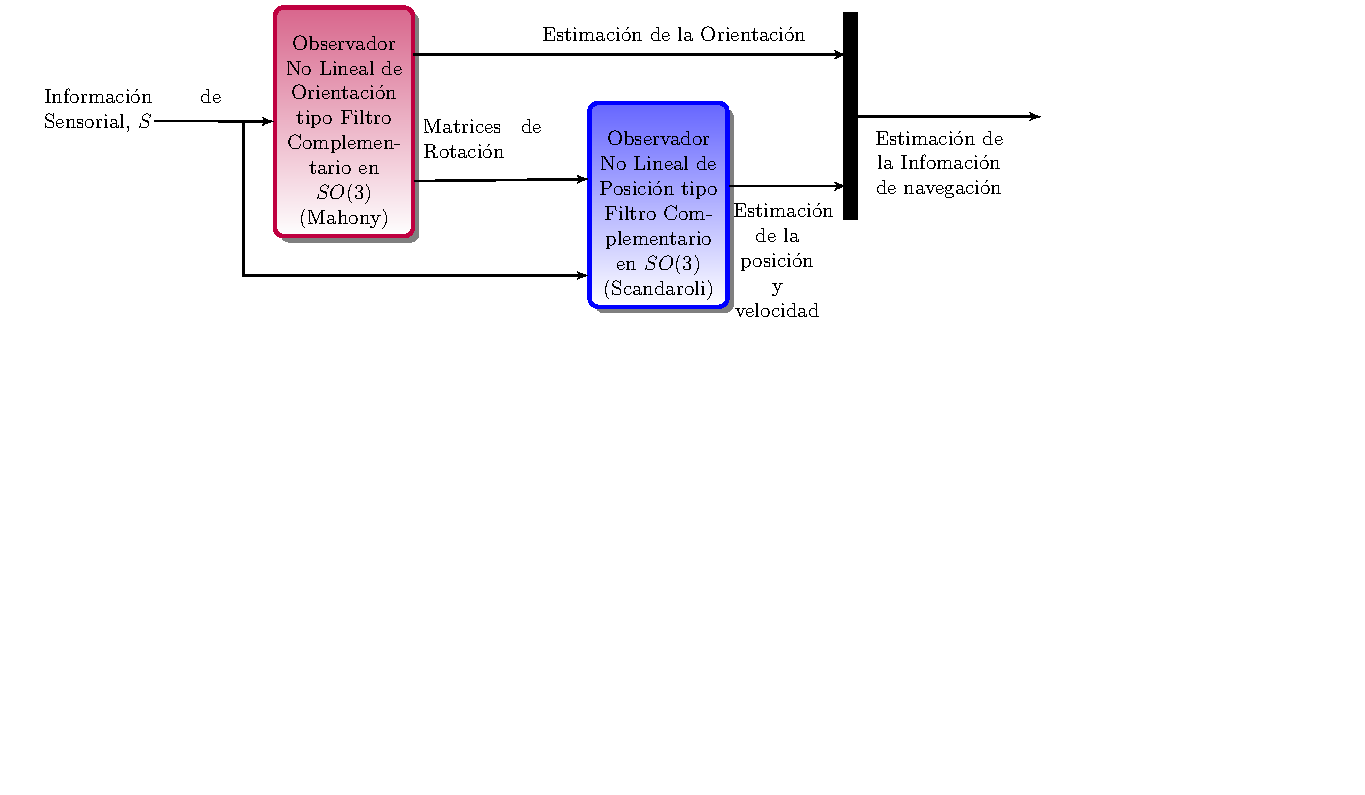
\includegraphics[scale=0.61,viewport=10 220 560 380,clip]{aam2.pdf}
\caption{Esquema simplificado del algoritmo de Mahony-Scandaroli.}
\scriptsize{Fuente: Elaboración Propia}
\label{solucionMS_fig1}
\end{center}
\end{figure}
El algoritmo de navegación de Mahony-Scandaroli, puede ser esquematizado tal como se muestra en la Figura \ref{solucionMS_fig1}. En este esquema, el observador orientación toma parte de la medición de los sensores de navegación (elementos del conjunto de \emph{información sensorial disponible} $S$) para estimar:
\begin{itemize}
\item La orientación en términos de los ángulos de Euler.
\item La velocidad angular en $\marco{B}$
\item El error de estimación de la matriz de rotación $\tilde{R}$, definida como la transformación $\marco{E}\hookrightarrow\marco{B}$, donde $\marco{E}$ denota el marco referencial de estimación definido a través del error de la estimación de la orientación en $SO(3)$.
\item Y la matriz $\hat{R}$ para $\marco{E}\hookrightarrow\marco{A}$.
\end{itemize}
En cascada, el observador de posición tipo Filtro complementario en SO(3), toma el resto de las variables incluidas en $S$ junto con las matrices de transformación determinadas por el anterior algoritmo, para obtener la estimación de la posición y su derivada en $\marco{A}$. Finalmente, los dos grupos de variables estimadas por ambos observadores conforman la \emph{estimación de la información de navegación}, que puede ser denotada por el vector columna $X=[\hat{p}~\hat{v}~\hat{\Theta}~\hat{\Omega}]$, donde $\hat{p}$ es la estimación de la posición en $\marco{A}$, $\hat{v}$ es la estimación de la velocidad en $\marco{A}$, $\hat{\Theta}$ es la estimación de la orientación en términos los ángulos de Euler, y $\hat{\Omega}$ es la estimación de la velocidad angular en $\marco{B}$.\par
%%
En resumen, el enfoque original del algoritmo de observadores en cascada de Mahony-Scandaroli, resuelve la determinación de la información de navegación en tres niveles de procesamiento:
a) la reconstrucción vectorial de la matriz de rotación $R_y$ usando la medición de un acelerómetro $a_s$ y un magnetómetro $m_s$\footnote{El desarrollo teórico y práctico de Mahony en [\cite{Mahony2008}] demuestra que no es absolutamente necesario incluir ambas mediciones. Y si el caso fuese de que alguna de las señales es demasiado ruidosa se puede prescindir de la misma.}; b) la determinación de la estimación de la velocidad angular $\hat{\omega}$, la estimación de la orientación en términos de los ángulos de Euler $\hat{\Theta}$, y la estimación de la matriz de rotación $\hat{R}$ con su respectivo error $\tilde{R}$\footnote{Definida como $\tilde{R}=R_y\hat{R}^T$}, los que se determinan usando las señales de la reconstrucción vectorial y la medición de un giroscopio $\Omega_s$; c) la determinación de la estimación de la posición $\hat{p}$, y la velocidad lineal $\hat{v}$ a partir de las anteriores salidas, es decir $\tilde{R}$ y $\hat{R}$, junto con la medición de posición $p_y$ y la aceleración $a_s$. 
%%%%%%%%%%%%%%
%%%%%%%%%%%%%%
%%%%%%%%%%%%%%
\section{Reconstrucción Óptima de la matriz de rotación}
Como señala Mahony, la principal desventaja en la formulación de los filtros complementarios pasivo y directo es la sensibilidad a la matriz de entrada $R_y$. Esta matriz es usada en el mapeo de la medición de la velocidad angular al marco inercial $\marco{A}$, y por esta razón, la determinación de esta matriz juega un papel central en el desempeño final del sistema.\par
%%
Considerando esto la determinación desde el enfoque de la reconstrucción vectorial del Mahony-Scandarolli, la recontrución sub-obtima basada en la resolucción de la ecuación de Lyapunov.
%%%%%%%%%%%%%%
%%%%%%%%%%%%%%
%%%%%%%%%%%%%%
\subsection{Determinacion de la matriz de rotación a partir de modelo de medición del vector gravitacional en cuaterniones}
\subsection{EKF dual del control óptimo}
\section{asa}
\cite{IEEEhowto:kopka}


\subsubsection{Subsubsection Heading Here}
Subsubsection text here.


% An example of a floating figure using the graphicx package.
% Note that \label must occur AFTER (or within) \caption.
% For figures, \caption should occur after the \includegraphics.
% Note that IEEEtran v1.7 and later has special internal code that
% is designed to preserve the operation of \label within \caption
% even when the captionsoff option is in effect. However, because
% of issues like this, it may be the safest practice to put all your
% \label just after \caption rather than within \caption{}.
%
% Reminder: the "draftcls" or "draftclsnofoot", not "draft", class
% option should be used if it is desired that the figures are to be
% displayed while in draft mode.
%
%\begin{figure}[!t]
%\centering
%\includegraphics[width=2.5in]{myfigure}
% where an .eps filename suffix will be assumed under latex, 
% and a .pdf suffix will be assumed for pdflatex; or what has been declared
% via \DeclareGraphicsExtensions.
%\caption{Simulation Results}
%\label{fig_sim}
%\end{figure}

% Note that IEEE typically puts floats only at the top, even when this
% results in a large percentage of a column being occupied by floats.


% An example of a double column floating figure using two subfigures.
% (The subfig.sty package must be loaded for this to work.)
% The subfigure \label commands are set within each subfloat command, the
% \label for the overall figure must come after \caption.
% \hfil must be used as a separator to get equal spacing.
% The subfigure.sty package works much the same way, except \subfigure is
% used instead of \subfloat.
%
%\begin{figure*}[!t]
%\centerline{\subfloat[Case I]\includegraphics[width=2.5in]{subfigcase1}%
%\label{fig_first_case}}
%\hfil
%\subfloat[Case II]{\includegraphics[width=2.5in]{subfigcase2}%
%\label{fig_second_case}}}
%\caption{Simulation results}
%\label{fig_sim}
%\end{figure*}
%
% Note that often IEEE papers with subfigures do not employ subfigure
% captions (using the optional argument to \subfloat), but instead will
% reference/describe all of them (a), (b), etc., within the main caption.


% An example of a floating table. Note that, for IEEE style tables, the 
% \caption command should come BEFORE the table. Table text will default to
% \footnotesize as IEEE normally uses this smaller font for tables.
% The \label must come after \caption as always.
%
%\begin{table}[!t]
%% increase table row spacing, adjust to taste
%\renewcommand{\arraystretch}{1.3}
% if using array.sty, it might be a good idea to tweak the value of
% \extrarowheight as needed to properly center the text within the cells
%\caption{An Example of a Table}
%\label{table_example}
%\centering
%% Some packages, such as MDW tools, offer better commands for making tables
%% than the plain LaTeX2e tabular which is used here.
%\begin{tabular}{|c||c|}
%\hline
%One & Two\\
%\hline
%Three & Four\\
%\hline
%\end{tabular}
%\end{table}


% Note that IEEE does not put floats in the very first column - or typically
% anywhere on the first page for that matter. Also, in-text middle ("here")
% positioning is not used. Most IEEE journals/conferences use top floats
% exclusively. Note that, LaTeX2e, unlike IEEE journals/conferences, places
% footnotes above bottom floats. This can be corrected via the \fnbelowfloat
% command of the stfloats package.



\section{Conclusion}
The conclusion goes here.




% conference papers do not normally have an appendix


% use section* for acknowledgement
\section*{Acknowledgment}


The authors would like to thank...





% trigger a \newpage just before the given reference
% number - used to balance the columns on the last page
% adjust value as needed - may need to be readjusted if
% the document is modified later
%\IEEEtriggeratref{8}
% The "triggered" command can be changed if desired:
%\IEEEtriggercmd{\enlargethispage{-5in}}

% references section

% can use a bibliography generated by BibTeX as a .bbl file
% BibTeX documentation can be easily obtained at:
% http://www.ctan.org/tex-archive/biblio/bibtex/contrib/doc/
% The IEEEtran BibTeX style support page is at:
% http://www.michaelshell.org/tex/ieeetran/bibtex/
\bibliographystyle{IEEEtran}
% argument is your BibTeX string definitions and bibliography database(s)
\bibliography{IEEEabrv,BiblioTh7}
%
% <OR> manually copy in the resultant .bbl file
% set second argument of \begin to the number of references
% (used to reserve space for the reference number labels box)
\printbibliography[title=Referencias]
%\begin{thebibliography}{10}
%
%\bibitem{IEEEhowto:kopka}
%H.~Kopka and P.~W. Daly, \emph{A Guide to \LaTeX}, 3rd~ed.\hskip 1em plus
%  0.5em minus 0.4em\relax Harlow, England: Addison-Wesley, 1999.
%
%\end{thebibliography}




% that's all folks
\end{document}


